\documentclass{beamer}

% for themes, etc.
\mode<presentation>
{ \usetheme{Torino} }
%{ \usetheme{boxes} }

\usepackage{times}  % fonts are up to you
\usepackage{graphicx}

% these will be used later in the title page
\title{ALICE MUON Software for run 3}
\author{Sean Murray \\
    Physics \\
    University of Cape Town 
}
\date{July 6, 2016}

% note: do NOT include a \maketitle line; also note that this title
% material goes BEFORE the \begin{document}

% have this if you'd like a recurring outline
\AtBeginSection[]  % "Beamer, do the following at the start of every section"
{
\begin{frame}<beamer> 
\frametitle{Outline} % make a frame titled "Outline"
\tableofcontents[currentsection]  % show TOC and highlight current section
\end{frame}
}

\begin{document}

% this prints title, author etc. info from above
\begin{frame}
\titlepage
\end{frame}

\section{ALICE}

\begin{frame}
\frametitle{ALICE}
Pick of alice\ldots.
\end{frame}

\begin{frame}
\frametitle{ALICE MUON Arm}
Pic of muon arm \ldots
\end{frame}

\begin{frame}
  \frametitle{ALICE MUON diagram}


\end{frame}

\begin{frame}
\frametitle{Detector Structure}
pic of detector slats 

\end{frame}

\begin{frame}
\frametitle{Detector Structure 2}
pic of wire chamber 

\end{frame}

\section{O2 and Run3}
\begin{frame}
\frametitle{O2 Online/Offline}


\end{frame}

\section{Current MUON Software}

\begin{frame}
\frametitle{Current MUON Software}


\begin{theorem}
The angles in a triangle sum to $180^{\circ}$.
\end{theorem}

\pause

Plan:  Extend AC past C to D.  Draw CE parallel to AB.

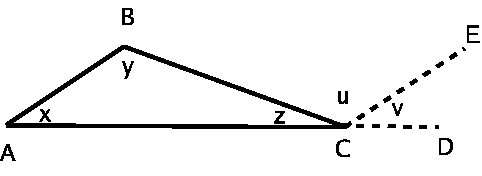
\includegraphics[width = 2.0in]{BeamerTriangle.jpg}  

\end{frame}

\begin{frame}

\begin{proof}

\begin{tabular}{ll}
% uncover makes advanced overlay
\uncover<1->{1. u = y} & \uncover<2->{Alternate angles of a
transveral.} \\ 
\uncover<3->{2. v = x} & \uncover<4->{Consecutive interior angles of a
transveral} \\ 
\uncover<5->{3. z+u+v = $180^{\circ}$} & \uncover<6->{ACD is a straight
line.} \\ 
\uncover<7->{4. z+y+x = $180^{\circ}$} & \uncover<8->{Substitution
from Steps 1 and 2.} \\
\end{tabular}

\end{proof}

\end{frame}

\section{Cluster Finder}

\begin{frame}
\frametitle{What is a cluster finder} 

\begin{itemize}

\item This tour just scratches the surface.  
\pause

\item {\sc beamer} has enough features to fill a 210-page user manual!  
\pause

\item Advanced example:
\url{http://latex-beamer.sourceforge.net/beamerexample1.pdf}.

\end{itemize}

\end{frame}

\end{document}

